\documentclass[answers]{exam}
\usepackage{../MT2024}
\usepackage{graphicx}
\graphicspath{ {./images/} }

\title{Probability -- Sheet 4\\Markov chains, Time reversal}
\author{YOUR NAME HERE :)}
\date{Michaelmas Term 2024}
% accurate as of 12/11/2024


\begin{document}
\maketitle

\begin{questions}

\question%1
Find the stationary distributions of the following transition matrices. In each case describe the limiting behaviour of $p_{12}^{(n)}$ as $n \to \infty$.
\begin{parts}
\part%1a
$\begin{pmatrix}
	0 & 0 & 1 \\
	0 & \frac{1}{2} & \frac{1}{2} \\
	\frac{1}{3} & \frac{1}{3} & \frac{1}{3}
\end{pmatrix}$;

\part%1b
$\begin{pmatrix}
	0 & \frac{1}{2} & \frac{1}{3} & \frac{1}{6} \\
	1 & 0 & 0 & 0 \\
	1 & 0 & 0 & 0 \\
	1 & 0 & 0 & 0
\end{pmatrix}$

\part%1c
$\begin{pmatrix}
	0 & \frac{1}{2} & 0 & \frac{1}{2} & 0 \\
	0 & \frac{1}{2} & \frac{1}{2} & 0 & 0 \\
	0 & \frac{1}{2} & \frac{1}{2} & 0 & 0 \\
	\frac{1}{2} & 0 & 0 & 0 & \frac{1}{2} \\
	0 & 0 & 0 & 0 & 1
\end{pmatrix}$
\end{parts}



\question%2
Let $X_{n}$ denote the sum of $n$ independent rolls of a fair six-sided die. Find \[
	\lim _{n \to \infty} \mathbb{P}(X_{n} \text { is a multiple of } 11).
\]



\question%3
A knight performs a random walk on a chessboard, making each possible move with equal probability at each step. (The knight's possible moves from two different positions are shown in the picture.)
\begin{center}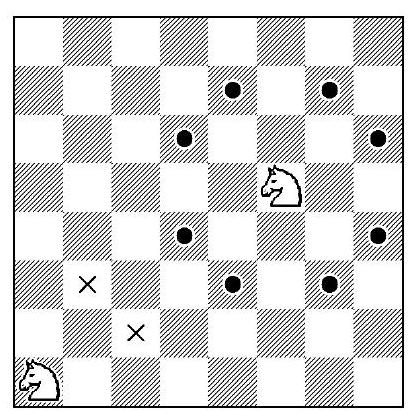
\includegraphics[width=5cm]{sheet 4 q 3}\end{center}
\begin{parts}
\part%3a
If the knight starts in the bottom left corner, how many moves on average will it take to return there? [\emph{Hint: consider the "random walk on a graph" from lectures, in which the equilibrium probability of a vertex is proportional to its number of neighbours.}]

\part%3b
Let $p_{n}$ be the probability that the knight is back in the same corner after $n$ steps. Describe the behaviour of $p_{n}$ as $n \to \infty$.
\end{parts}



\question%4
A fair six-sided die is rolled repeatedly. On average how long does it take until the first time that the product of the numbers rolled is a square? (For example, if the first roll is 1 or 4, it takes just one roll; if the sequence begins $3,2,6$, then it takes three rolls.)



\question%5
A frog jumps on an infinite ladder. At each jump, with probability $1-p$ he jumps up one step, while with probability $p$ he slips off and falls all the way to the bottom.
\begin{parts}
\part%5a
Give the transition probabilities for a Markov chain representing the frog's height on the ladder after each jump.

\part%5b
Show that the stationary distribution is geometric, and find its parameter.

\part%5c
Use the ergodic theorem to obtain a precise statement about the long-run proportion of time for which the frog is on the first step above the bottom of the ladder.

\part%5d
If the frog has just fallen to the bottom, on average how many jumps will it take before he next reaches step $k$? (One approach: consider the mean return time from $k$ to itself.)

\part%5e
Describe the time-reversal of the chain in equilibrium.
\end{parts}



\question%6
Let $P$ be the Markov transition matrix $\begin{pmatrix}0 & \frac{1}{2} & \frac{1}{2} \\ 1-p & 0 & p \\ 1-q & q & 0\end{pmatrix}$. For which $p$ and $q$ in $(0,1)$ is the matrix time-reversible? [\emph{Hint: You don't need to find the stationary distribution in the general case. It's enough to consider the detailed balance equations.}]



\question%7
Let $P=(p_{i j})$ be an irreducible transition matrix, and let $\pi$ be any positive probability distribution on the same state-space. Define a new transition matrix $Q$ by $q_{i j}=$ $\min (p_{i j}, p_{j i} \pi_{j} / \pi_{i})$ for $i \neq j$, with diagonal entries chosen so that the row sums are 1. Suppose $Q$ is irreducible. Show that $Q$ is reversible and has stationary distribution $\pi$. [\emph{This is a version of the Hastings-Metropolis algorithm. It constructs a Markov chain that converges to distribution $\pi$ -- a key point is that it can be operated using only some function proportional to $\pi$, rather than requiring the calculation of the normalised probability distribution $\pi$ itself.}]



\question%8
A professor owns $N$ umbrellas. She goes on two walks every day, one each morning to work and one each evening back home. On each walk, if she has an umbrella available, she carries one if and only if it is raining. If it is raining and there is no umbrella available, she walks anyway and gets wet. Suppose it is raining independently on each walk with probability $p$. What is the long-run proportion of walks on which she gets wet? [\emph{Hint: define a Markov chain to represent the number of umbrellas at home at the end of each day.}]



\question%9
Consider the following unreliable sorting process. We have $n$ objects labelled $1,2, \ldots, n$, arranged in some order. At each step, choose $i \in\{1,2, \ldots, n-1\}$ uniformly at random. Then sort the objects currently in positions $i$ and $i+1$ into increasing order with probability $1 /(1+q)$ and into decreasing order with probability $q /(1+q)$. Here $q \in(0,1)$ is some fixed parameter. Consider the process as a Markov chain, on the state space $S_{n}$ (the set of permutations of $n$ objects) of size $n!$. For distinct permutations $\alpha, \beta \in S_{n}$, the transition probability $p_{\alpha, \beta}$ is either $\frac{1}{n-1} \frac{1}{1+q}$, or $\frac{1}{n-1} \frac{q}{1+q}$, or 0.
\begin{parts}
\part%9a
Show that the chain is reversible in equilibrium. [\emph{Hint: the number of inversions of a permutation $\sigma$, denoted $\operatorname{inv}(\sigma)$, is the number of pairs $(i, j)$ for which $i<j$ and $\sigma_{i}>\sigma_{j}$. For example, the permutation $(24135) \in S_{5}$ has 3 inversions: it has each of the pairs $(1,2)$, $(1,4)$, and $(3,4)$ ``inverted". Note that any time the chain jumps from one state to another, the number of inversions either increases by 1 or decreases by 1. What do the detailed balance equations imply about the ratio between the probabilities of the two states?}]

\part%9b
In the stationary distribution, which are the most and least likely states, and what is the ratio of their probabilities? [\emph{To answer this, it's enough to know the stationary distribution up to a multiplicative constant.}]

\part%9c
(Optional.) Find an expression for the probability of the most likely state. [\emph{Now we need to know the multiplicative constant!}]
\end{parts}



\section*{Additional problem:}

\question%10
(\emph{An algebraic approach to convergence to equilibrium for reversible chains.}) We will use the Spectral Theorem for real symmetric matrices, which tells us that if $A$ is a real $m \times m$ symmetric matrix, then all its eigenvalues are real, and there exists an orthonormal basis of $\mathbb{R}^{m}$ consisting of eigenvectors of $A$. Let $P$ be an irreducible aperiodic reversible transition matrix on the finite state space $\{1,2, \ldots, m\}$, with stationary distribution $\pi$.
\begin{parts}
\part%10a
Let $D_{\pi}$ be the diagonal matrix with diagonal entries $\pi_{1}, \ldots, \pi_{m}$. Define a matrix $A=D_{\pi}^{1 / 2} P D_{\pi}^{-1 / 2}$, i.e. $A_{i j}=\pi_{i}^{1 / 2} \pi_{j}^{-1 / 2} P_{i j}$. Show that $A$ is symmetric.

\part%10b
Let $\phi^{(1)}, \phi^{(2)}, \ldots, \phi^{(n)}$ be an orthonormal basis of eigenvectors of $A$, with real eigenvalues $\lambda_{1} \geq \lambda_{2} \geq \cdots \geq \lambda_{n}$. Show that $f^{(j)}=D_{\pi}^{-1 / 2} \phi^{(j)}$ is an eigenvector of $P$ with eigenvalue $\lambda_{j}$. Deduce (using Q7 of Sheet 3) that $\lambda_{1}=1$ and $\left|\lambda_{j}\right|<1$ for $j \neq 1$.

\part%10c
Show that for any vector $f$, $P^{n} f$ converges as $n \to \infty$.

\part%10d
By considering an appropriate $f$, show that $(P^{n})_{i j} \to \pi_{j}$ as $n \to \infty$.

\part%10e
What can you say about the speed of convergence? [\emph{Consider $\beta=\max \left(\left|\lambda_{2}\right|,\left|\lambda_{n}\right|\right)$, the largest absolute value of an eigenvalue other than 1.}]
\end{parts}

\end{questions}

\end{document}
